\documentclass[12pt]{article}


\usepackage{amssymb}
\usepackage{amsmath}
\usepackage{fullpage}
\usepackage{epsfig}
\usepackage{epstopdf}
\everymath{\displaystyle}
\usepackage{enumerate}

\newif\ifans

\anstrue

\begin{document}

\begin{center}
\underline{\LARGE{Chapter 3.8: Graphs of the Trigonometric Functions}}
\end{center}

\subsection*{Expected Skills:}

\begin{itemize}

\item Be able to graph the trigonometric functions.

\end{itemize}

\subsection*{Practice Problems: }

\begin{enumerate}

\item Sketch the given function on the interval $[-2\pi,2\pi]$.  Label all asymptotes, intercepts with the coordinate axes, and local extrema.

\begin{enumerate}

\item $\displaystyle y=\sin{x}$

\ifans \fbox{\begin{tabular}{l}
$x$ intercepts: $\displaystyle \left(0,0 \right)$, $\displaystyle \left(\pm \pi,0 \right)$, and $\displaystyle \left(\pm 2\pi,0 \right)$\\
$y$ intercept: $(0,0)$\\
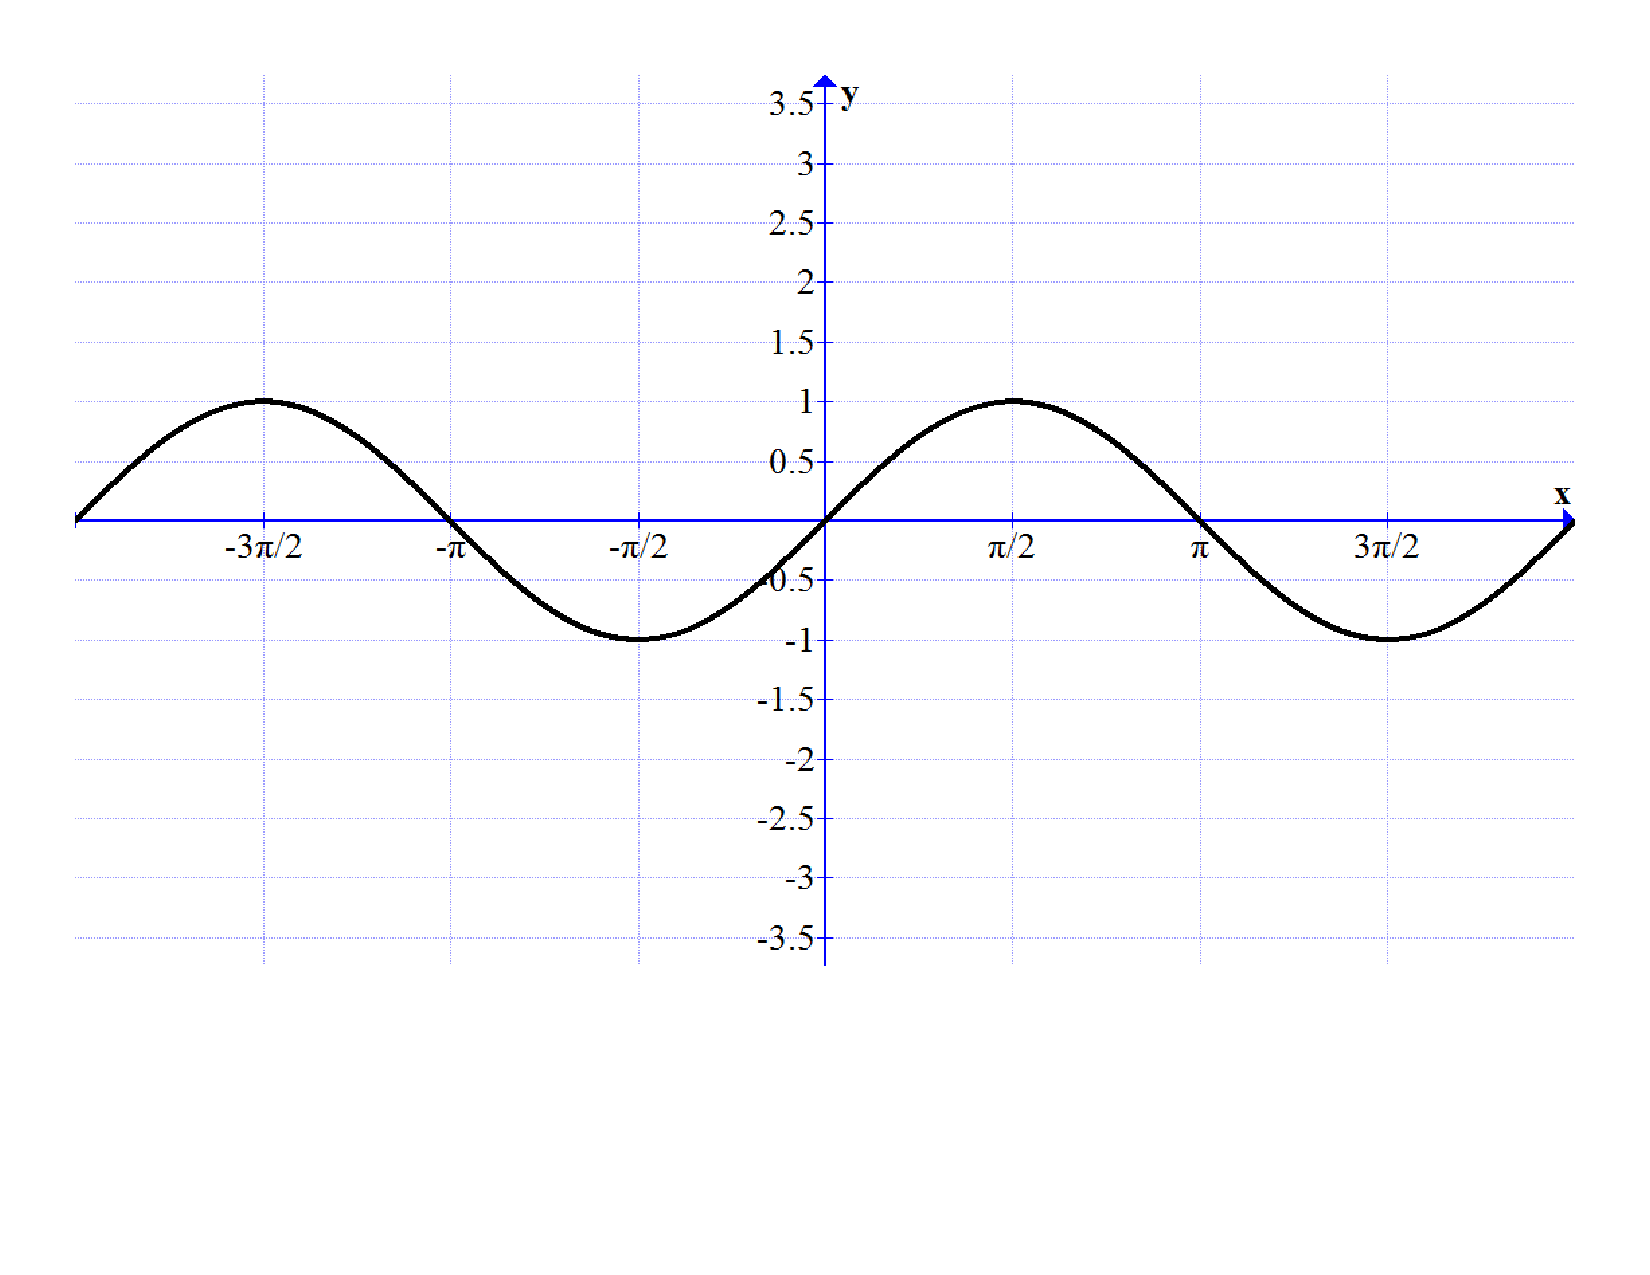
\includegraphics[scale=0.3]{sine.pdf}
\end{tabular}
} \fi

\item $\displaystyle y=\cos{x}$

\ifans \fbox{\begin{tabular}{l}
$x$ intercepts: $\displaystyle \left(\pm\frac{\pi}{2},0 \right)$ and $\displaystyle \left(\pm \frac{3\pi}{2},0 \right)$\\
$y$ intercept: $(0,1)$\\
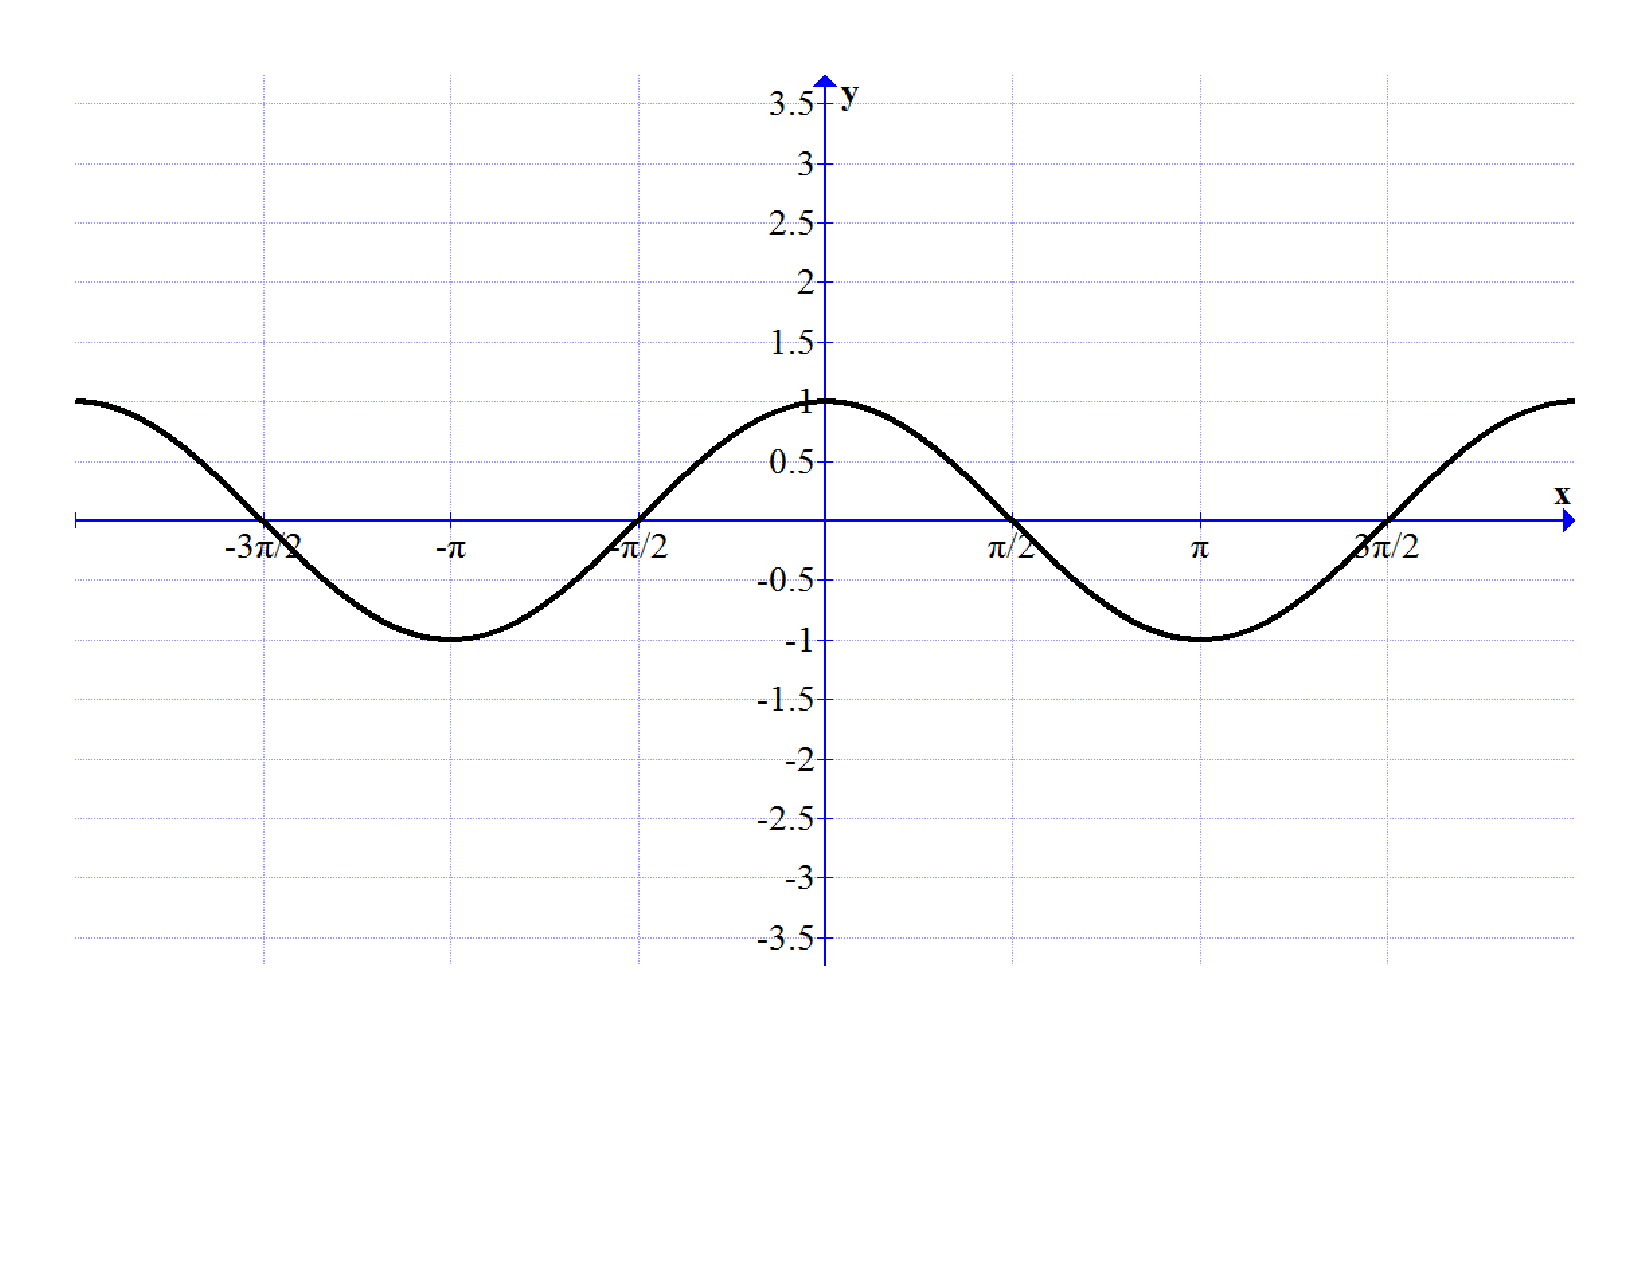
\includegraphics[scale=0.3]{cosine.pdf}
\end{tabular}
} \fi

\newpage

\item $\displaystyle y=\tan{x}$

\ifans \fbox{\begin{tabular}{l}
$x$ intercepts: $\displaystyle \left(0,0 \right)$, $\displaystyle \left(\pm \pi,0 \right)$ and $\displaystyle \left(\pm 2\pi,0 \right)$\\
$y$ intercept: $(0,0)$\\
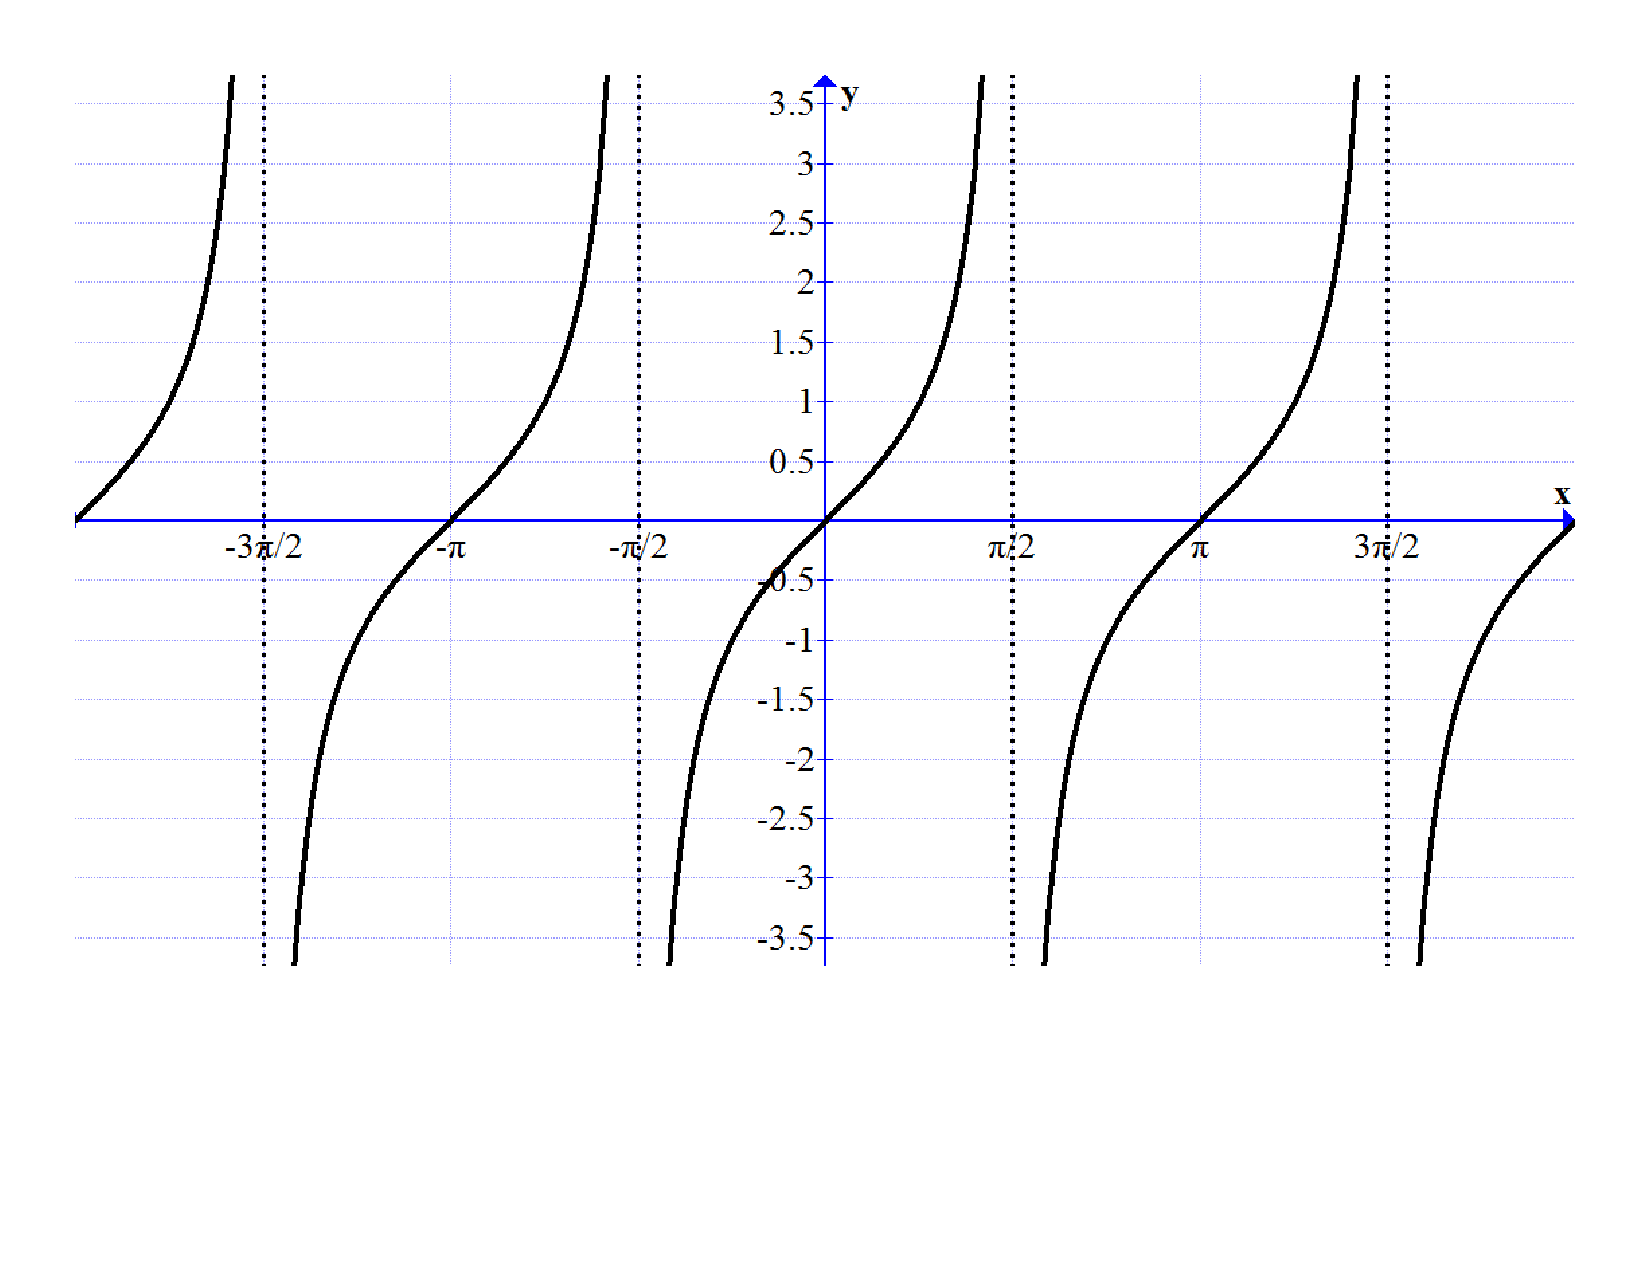
\includegraphics[scale=0.3]{tangent.pdf}
\end{tabular}
} \fi

\item $\displaystyle y=\cot{x}$

\ifans \fbox{\begin{tabular}{l}
$x$ intercepts: $\displaystyle \left(\pm \frac{\pi}{2},0 \right)$ and $\displaystyle \left(\pm \frac{3\pi}{2},0 \right)$\\
No $y$ intercept\\
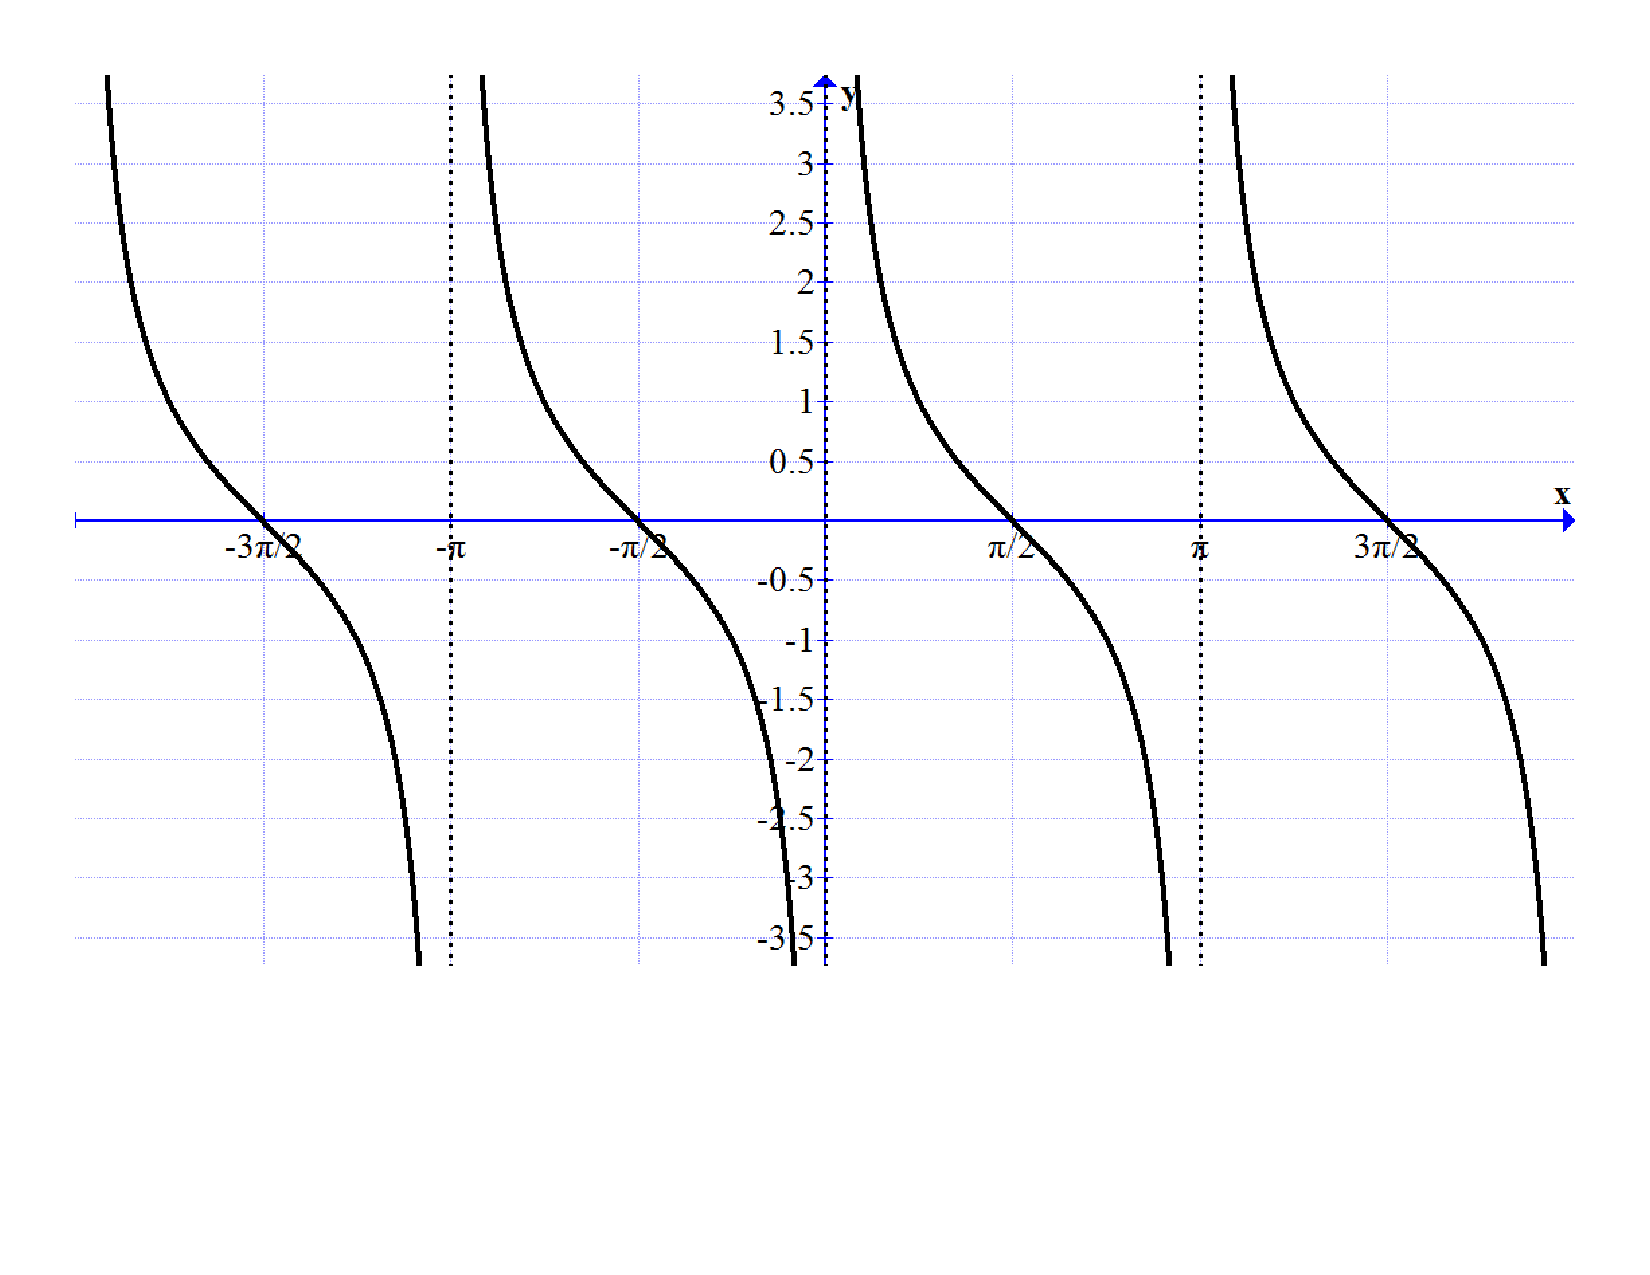
\includegraphics[scale=0.3]{cotangent.pdf}
\end{tabular}
} \fi

\item $\displaystyle y=\sec{x}$

\ifans \fbox{\begin{tabular}{l}
No $x$ intercepts, $y$ intercept: $(0,1)$\\
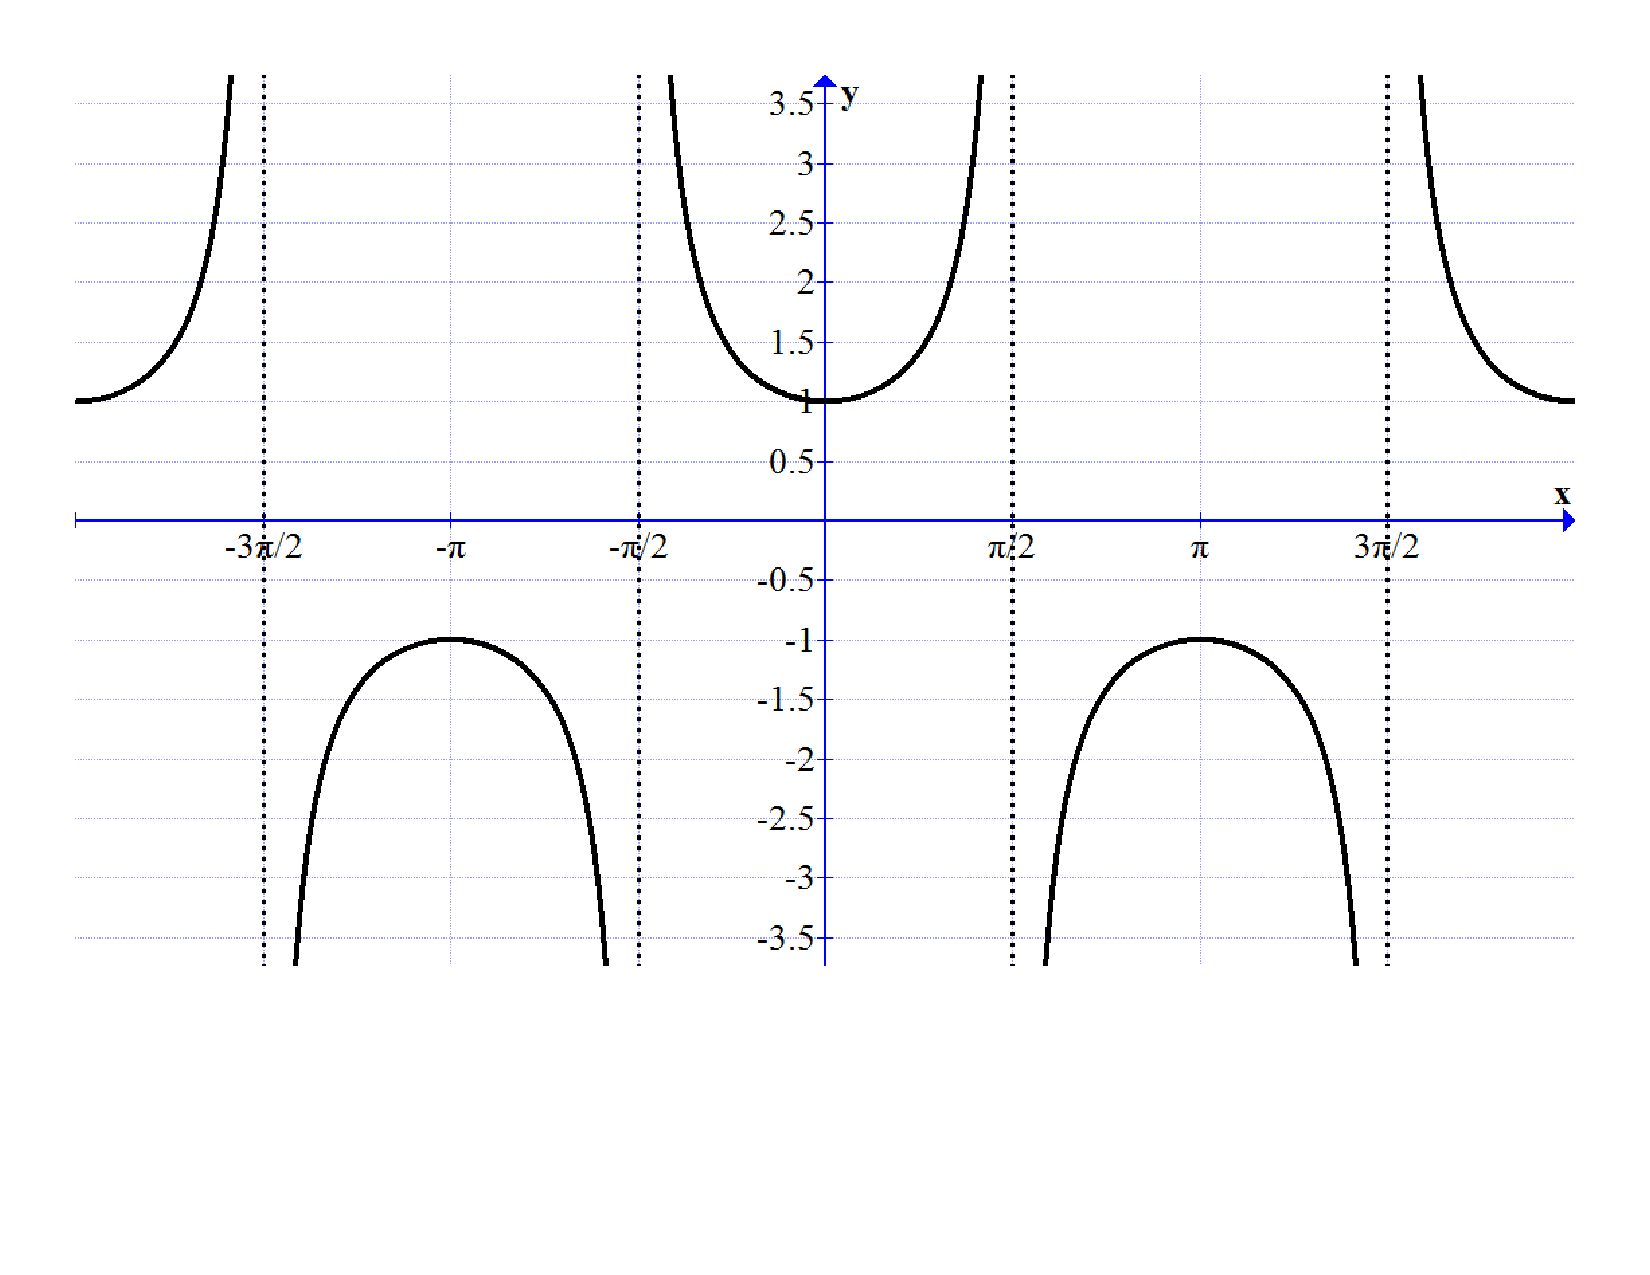
\includegraphics[scale=0.3]{secant.pdf}
\end{tabular}
} \fi

\newpage

\item $\displaystyle y=\csc{x}$

\ifans \fbox{\begin{tabular}{l}
No $x$ intercepts and no $y$ intercept\\
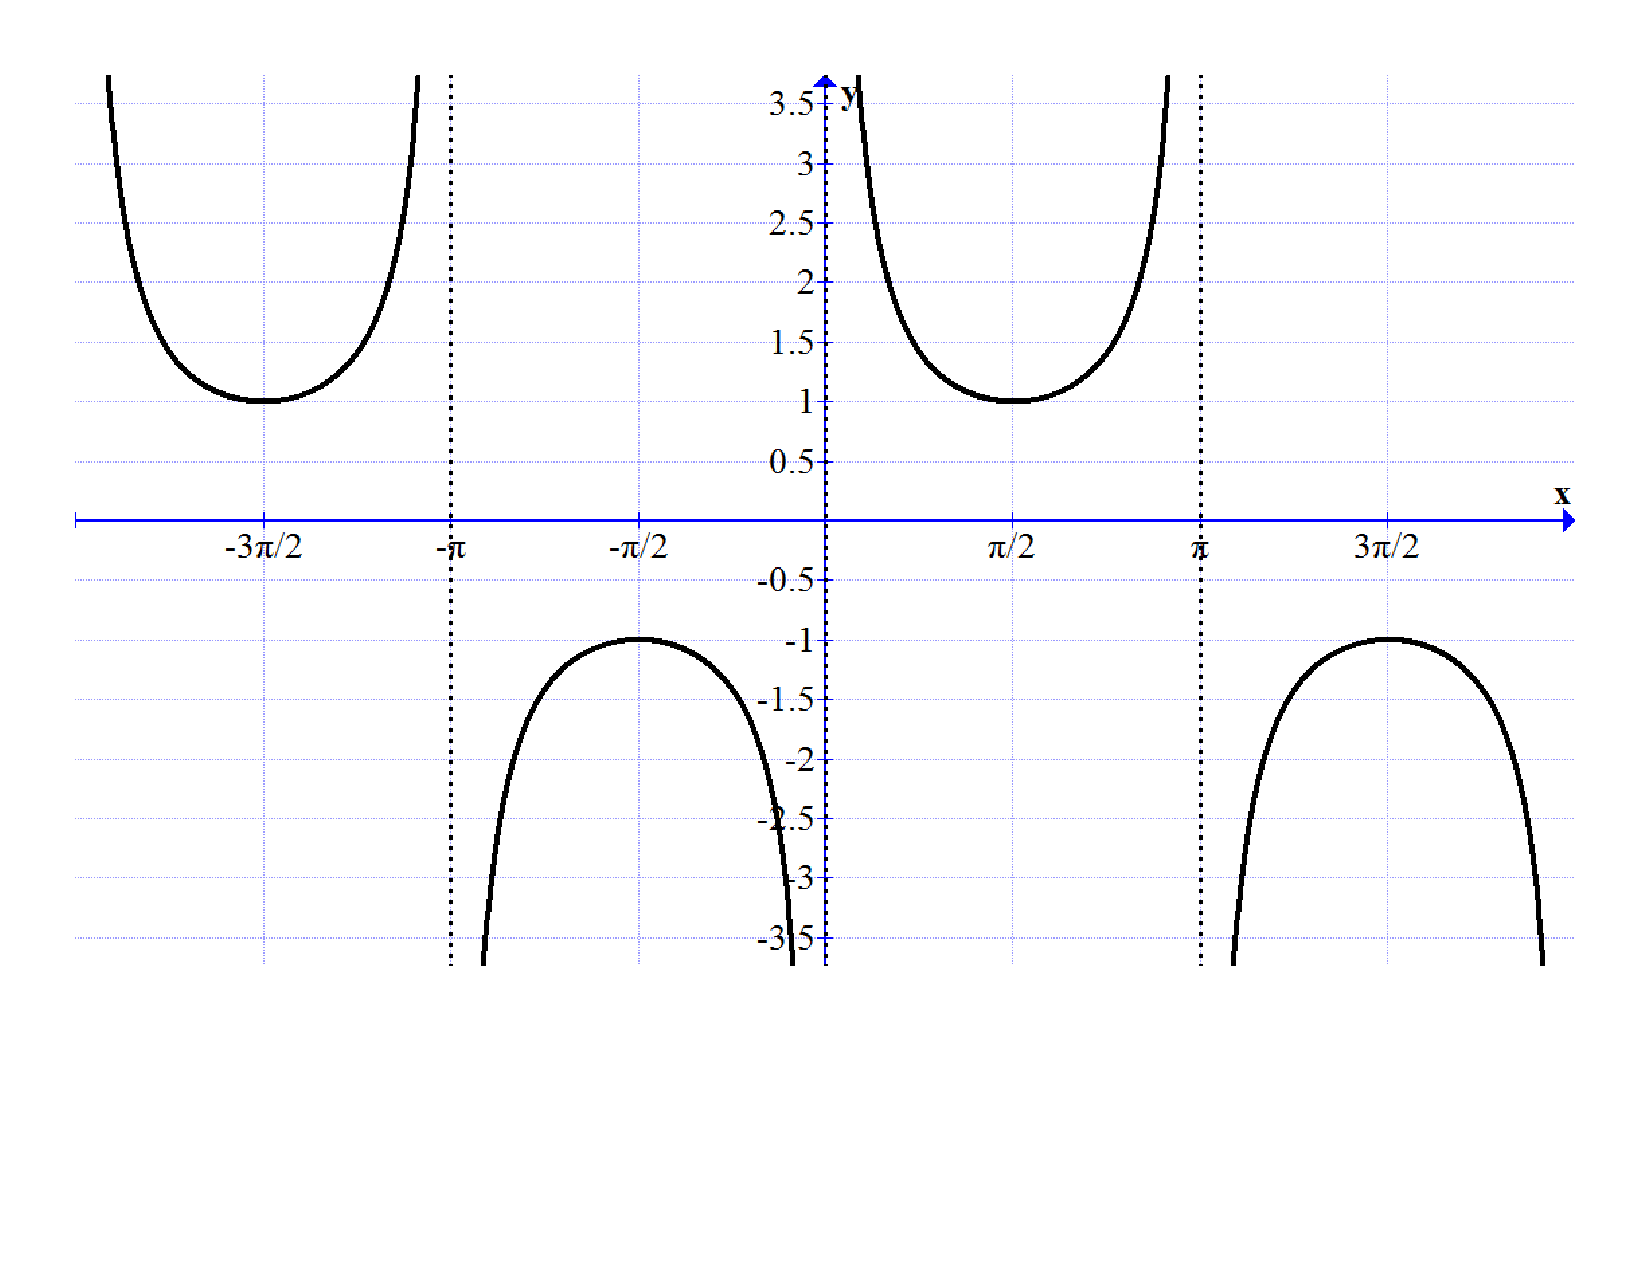
\includegraphics[scale=0.3]{cosecant.pdf}
\end{tabular}
} \fi

\end{enumerate}

\item Sketch each of the following functions on the interval $[0,2\pi]$.  Label all asymptotes, intercepts with the coordinate axes, and local extrema.  Also, determine the period.

\begin{enumerate}

\item $y=\cos{(3x)}$

\ifans\fbox{\parbox{0.6\linewidth}{The period is $\frac{2\pi}{3}$\\
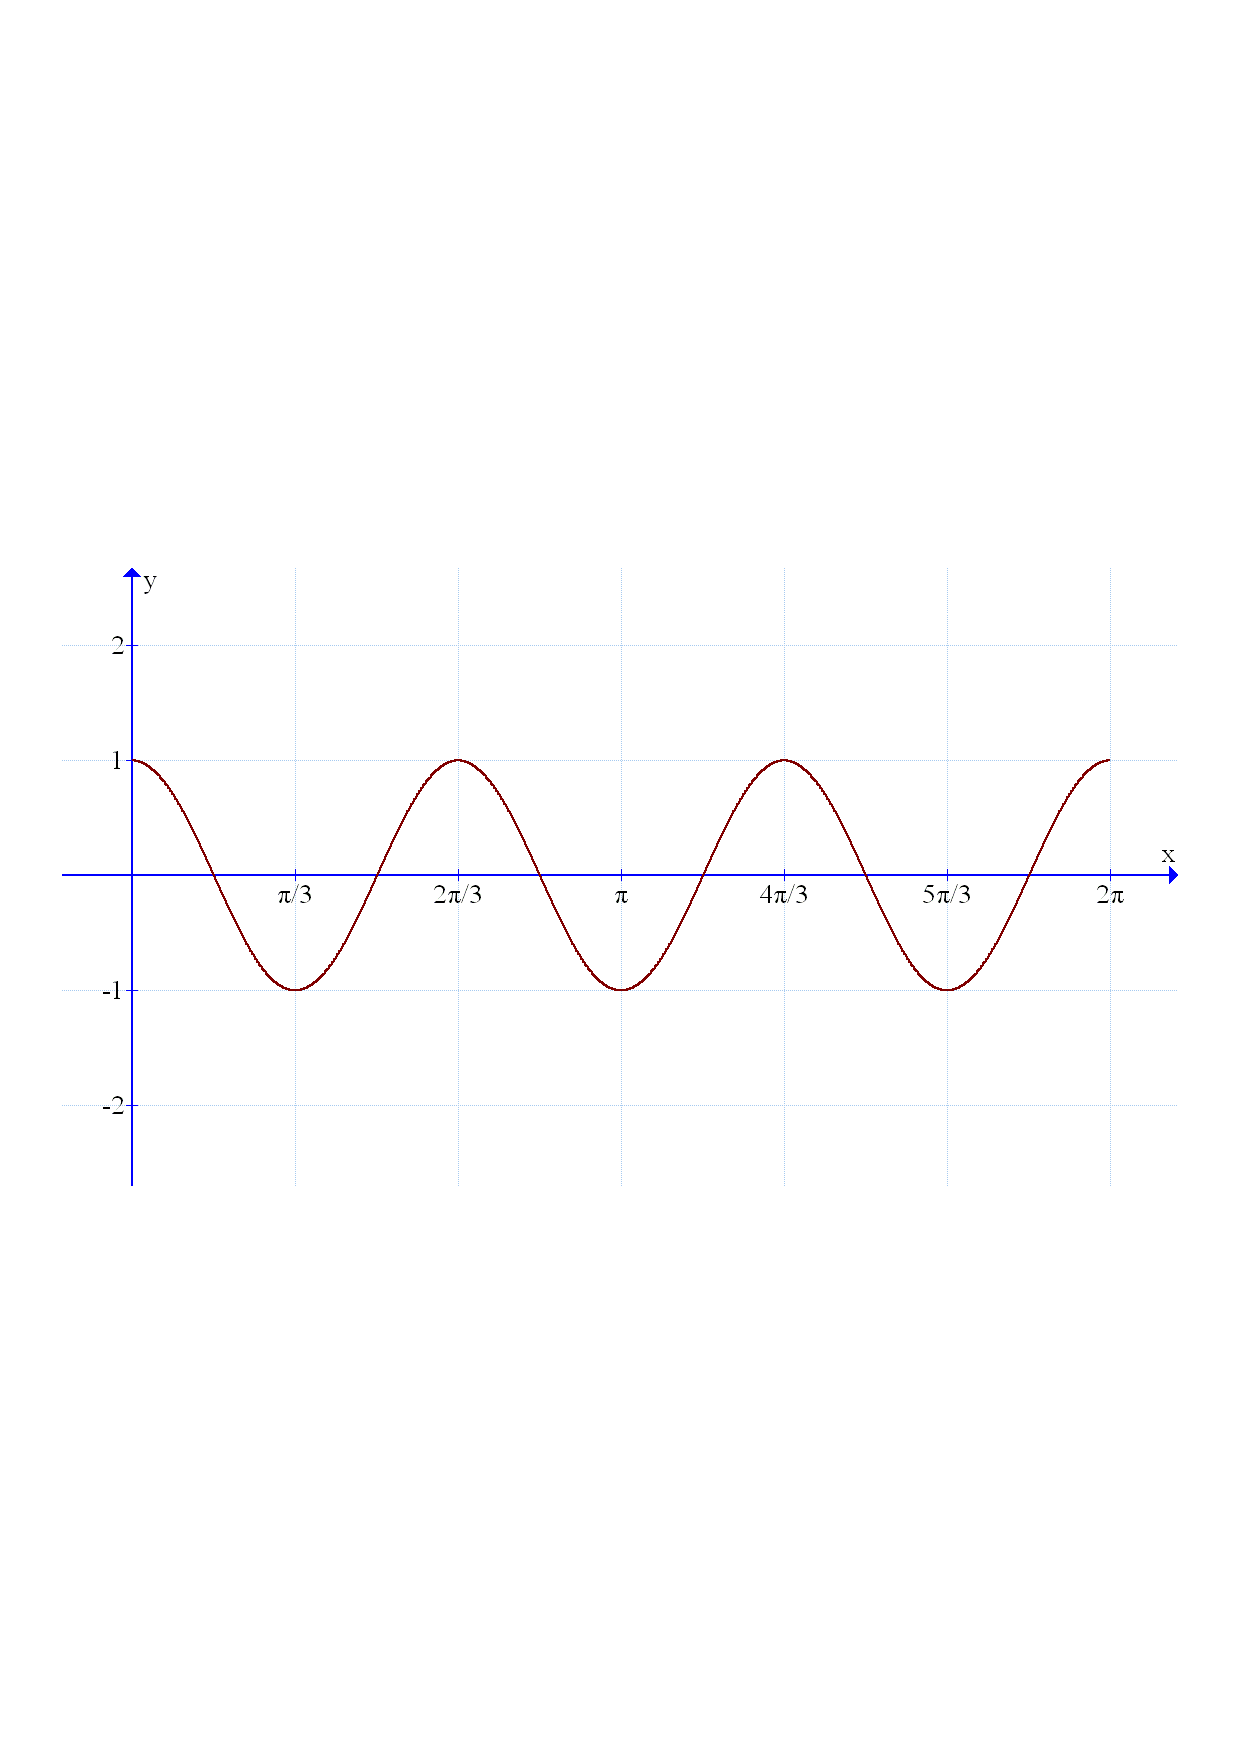
\includegraphics[scale=0.45]{cos3x.pdf}}} \fi

\item $y=3\sin{\left(\frac{x}{2}\right)}$

\ifans\fbox{\parbox{0.6\linewidth}{The period is $4\pi$\\
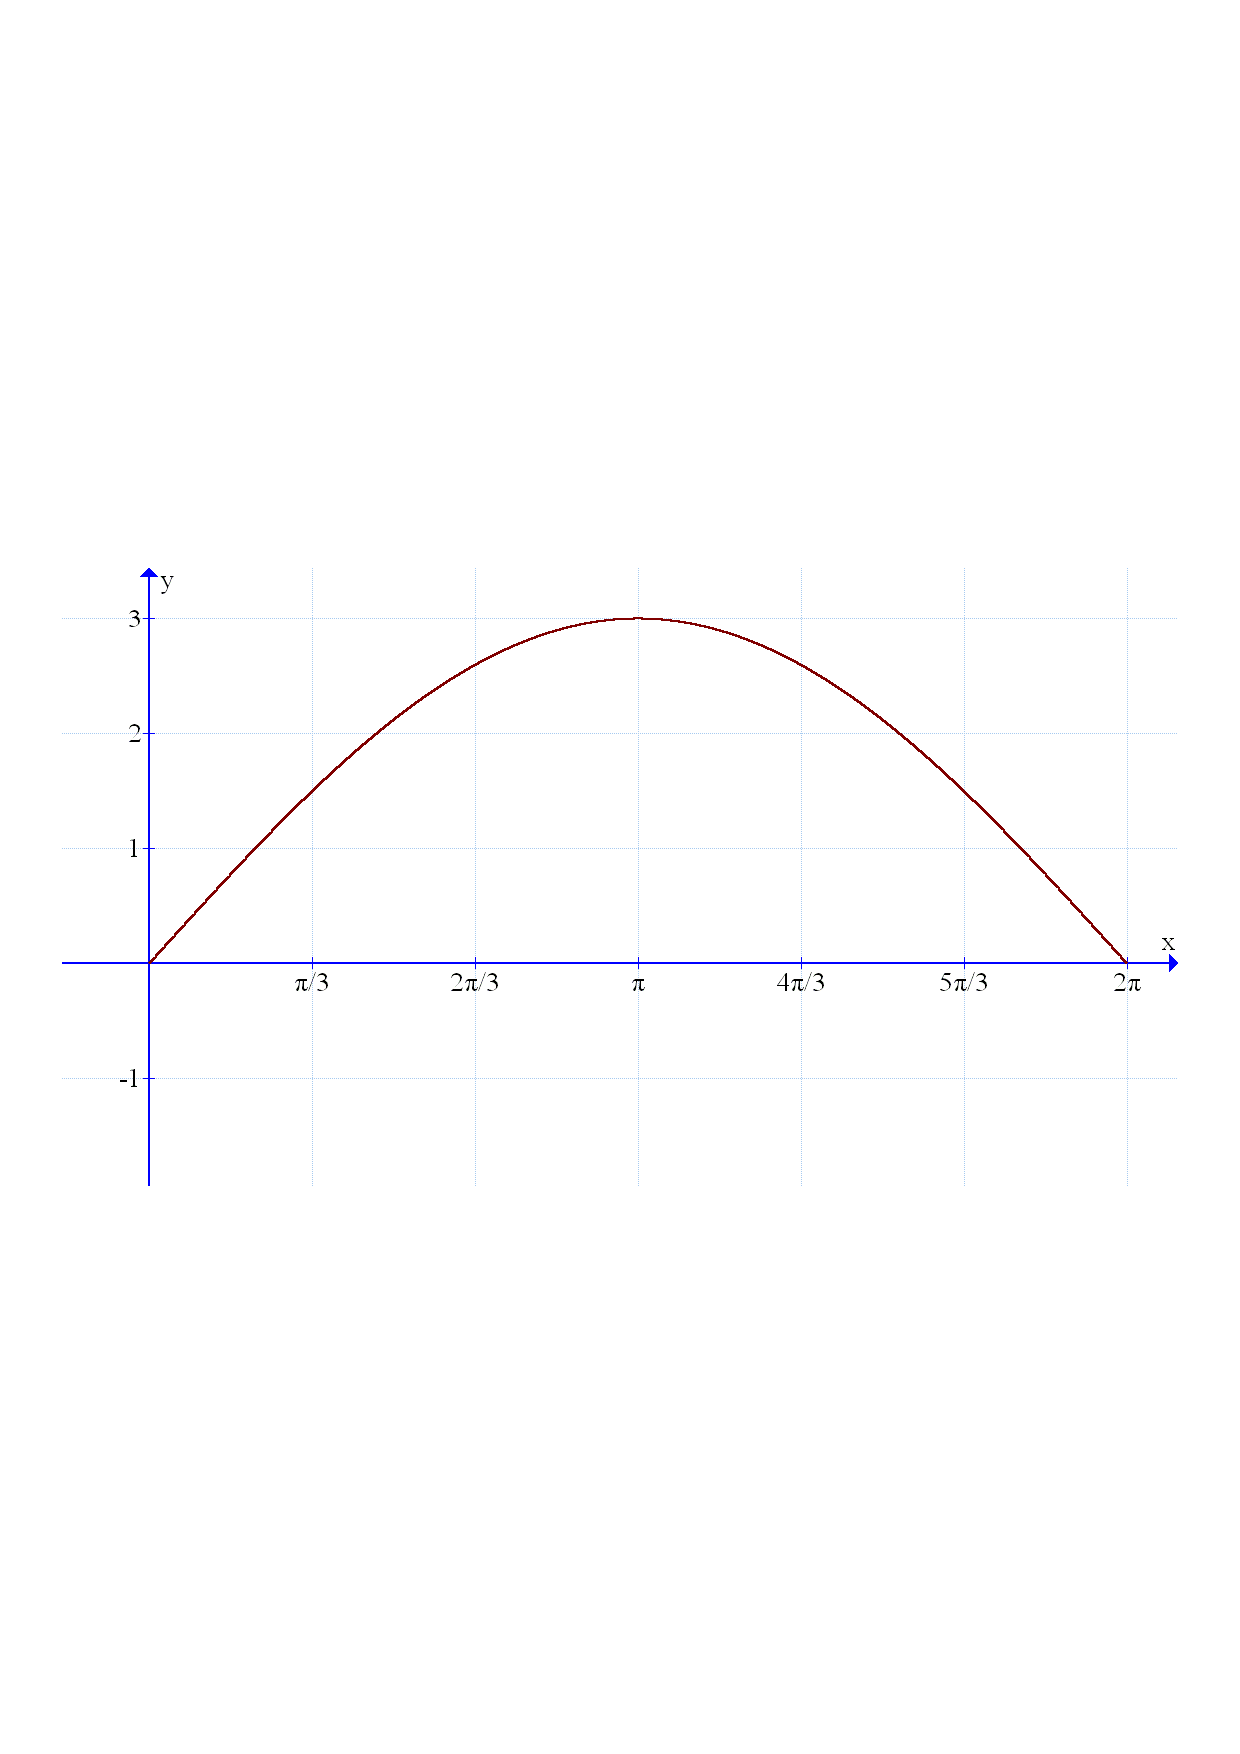
\includegraphics[scale=0.45]{sinx2.pdf}}} \fi

\newpage

\item $y=\frac{1}{2}\tan{\left(x\right)}$

\ifans\fbox{\parbox{0.7\linewidth}{The period is $\pi$\\
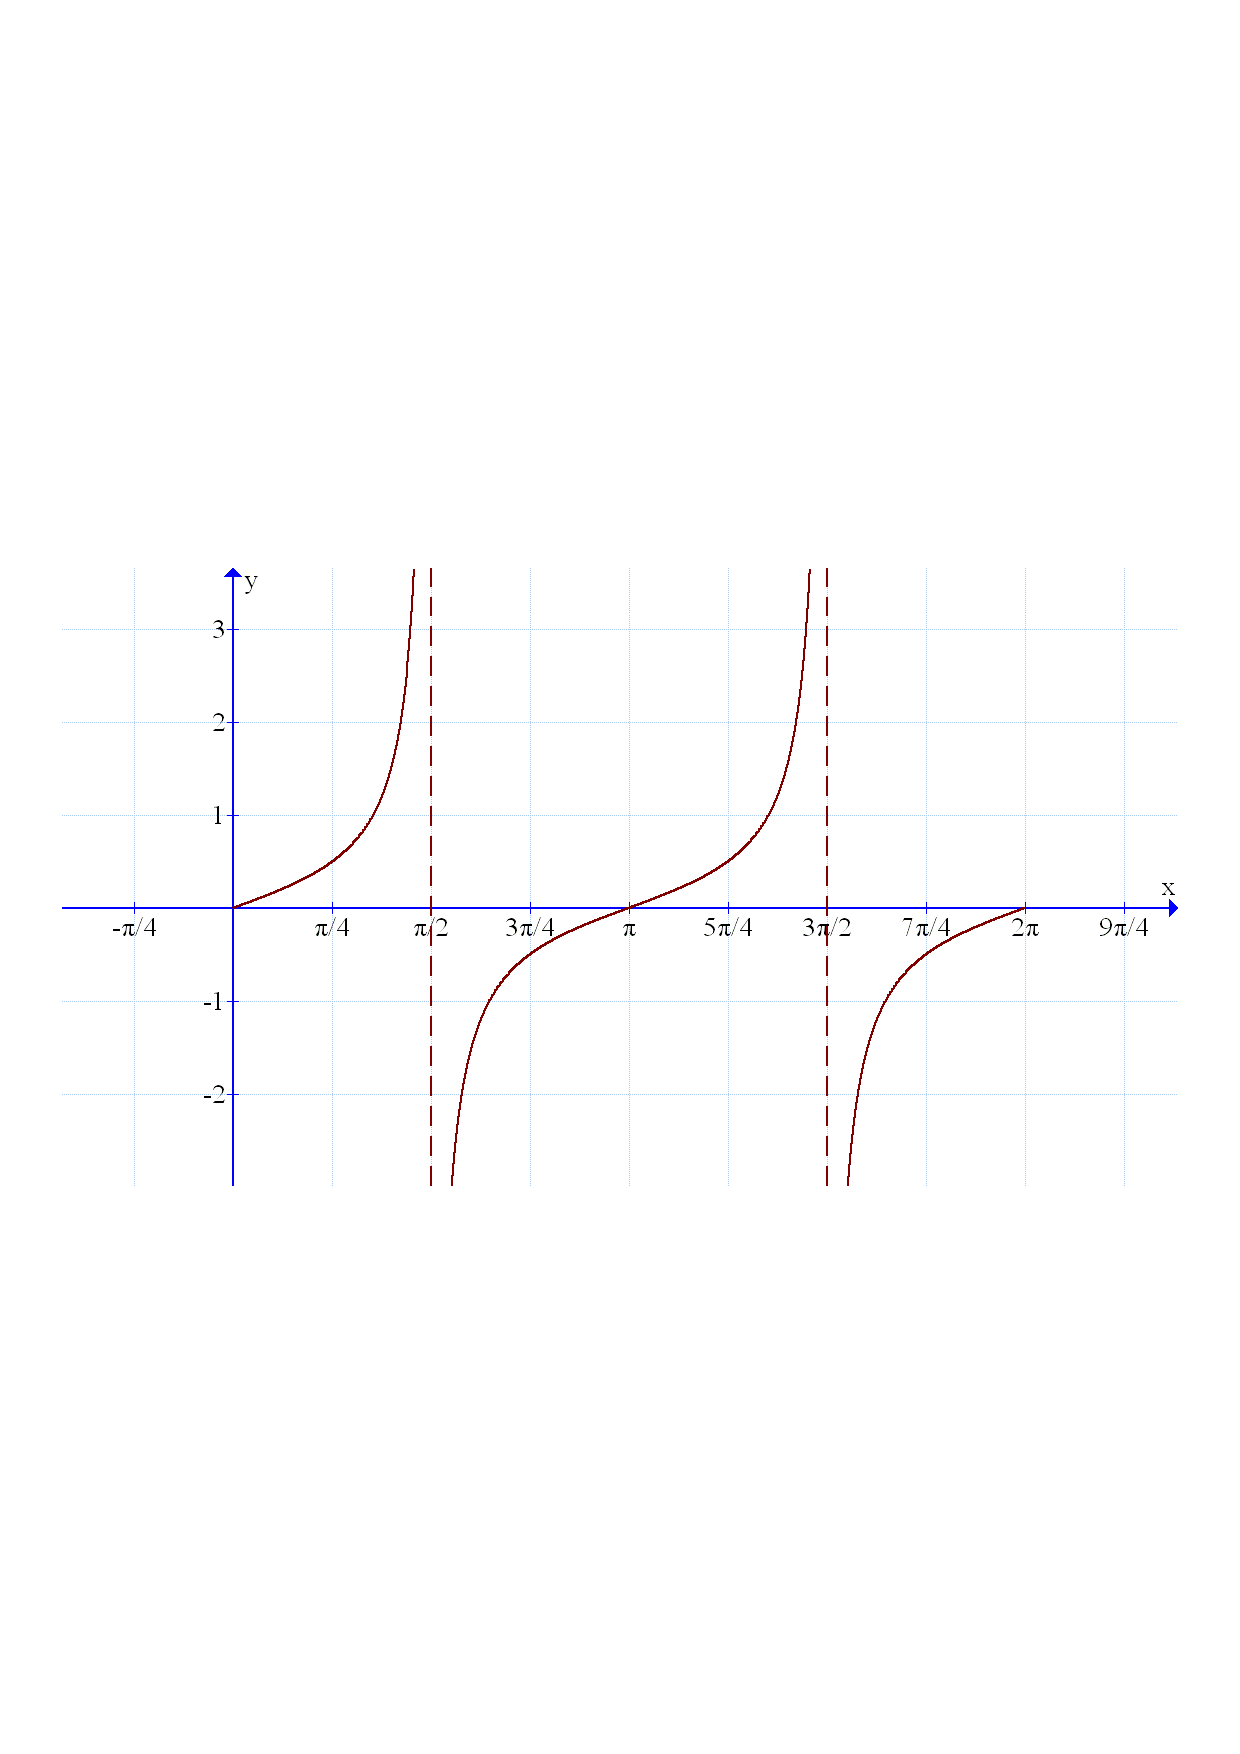
\includegraphics[scale=0.5]{0_5tanx.pdf}}} \fi

\item $y=\tan{\left(\frac{x}{2}\right)}$

\ifans\fbox{\parbox{0.7\linewidth}{The period is $2\pi$\\
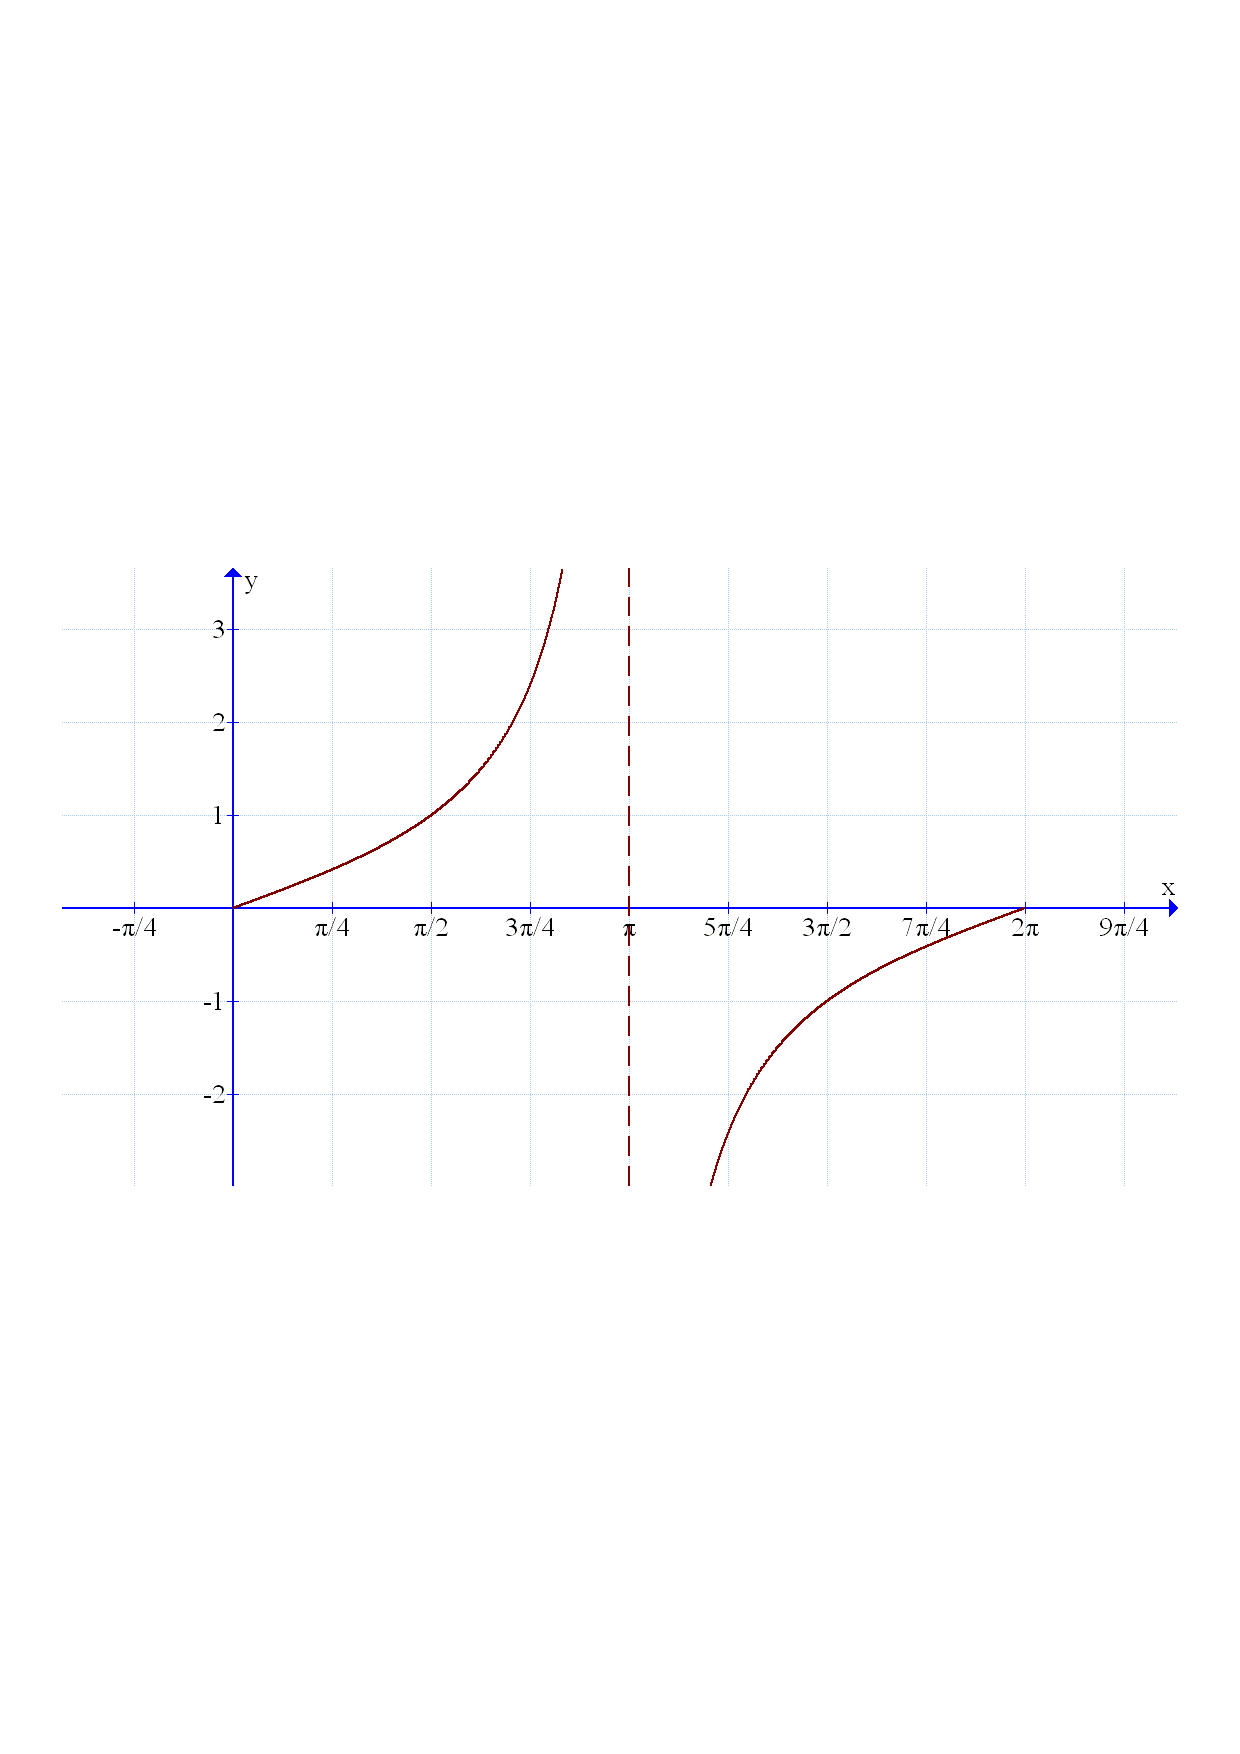
\includegraphics[scale=0.5]{tanx2.pdf}}} \fi

\end{enumerate}

\item Sketch the region in the $xy$-plane which is enclosed by $y=\sin{x}$ and $y=2-\sin{x}$ for $\frac{\pi}{2}\leq x \leq \frac{5\pi}{2}$.

\ifans\fbox{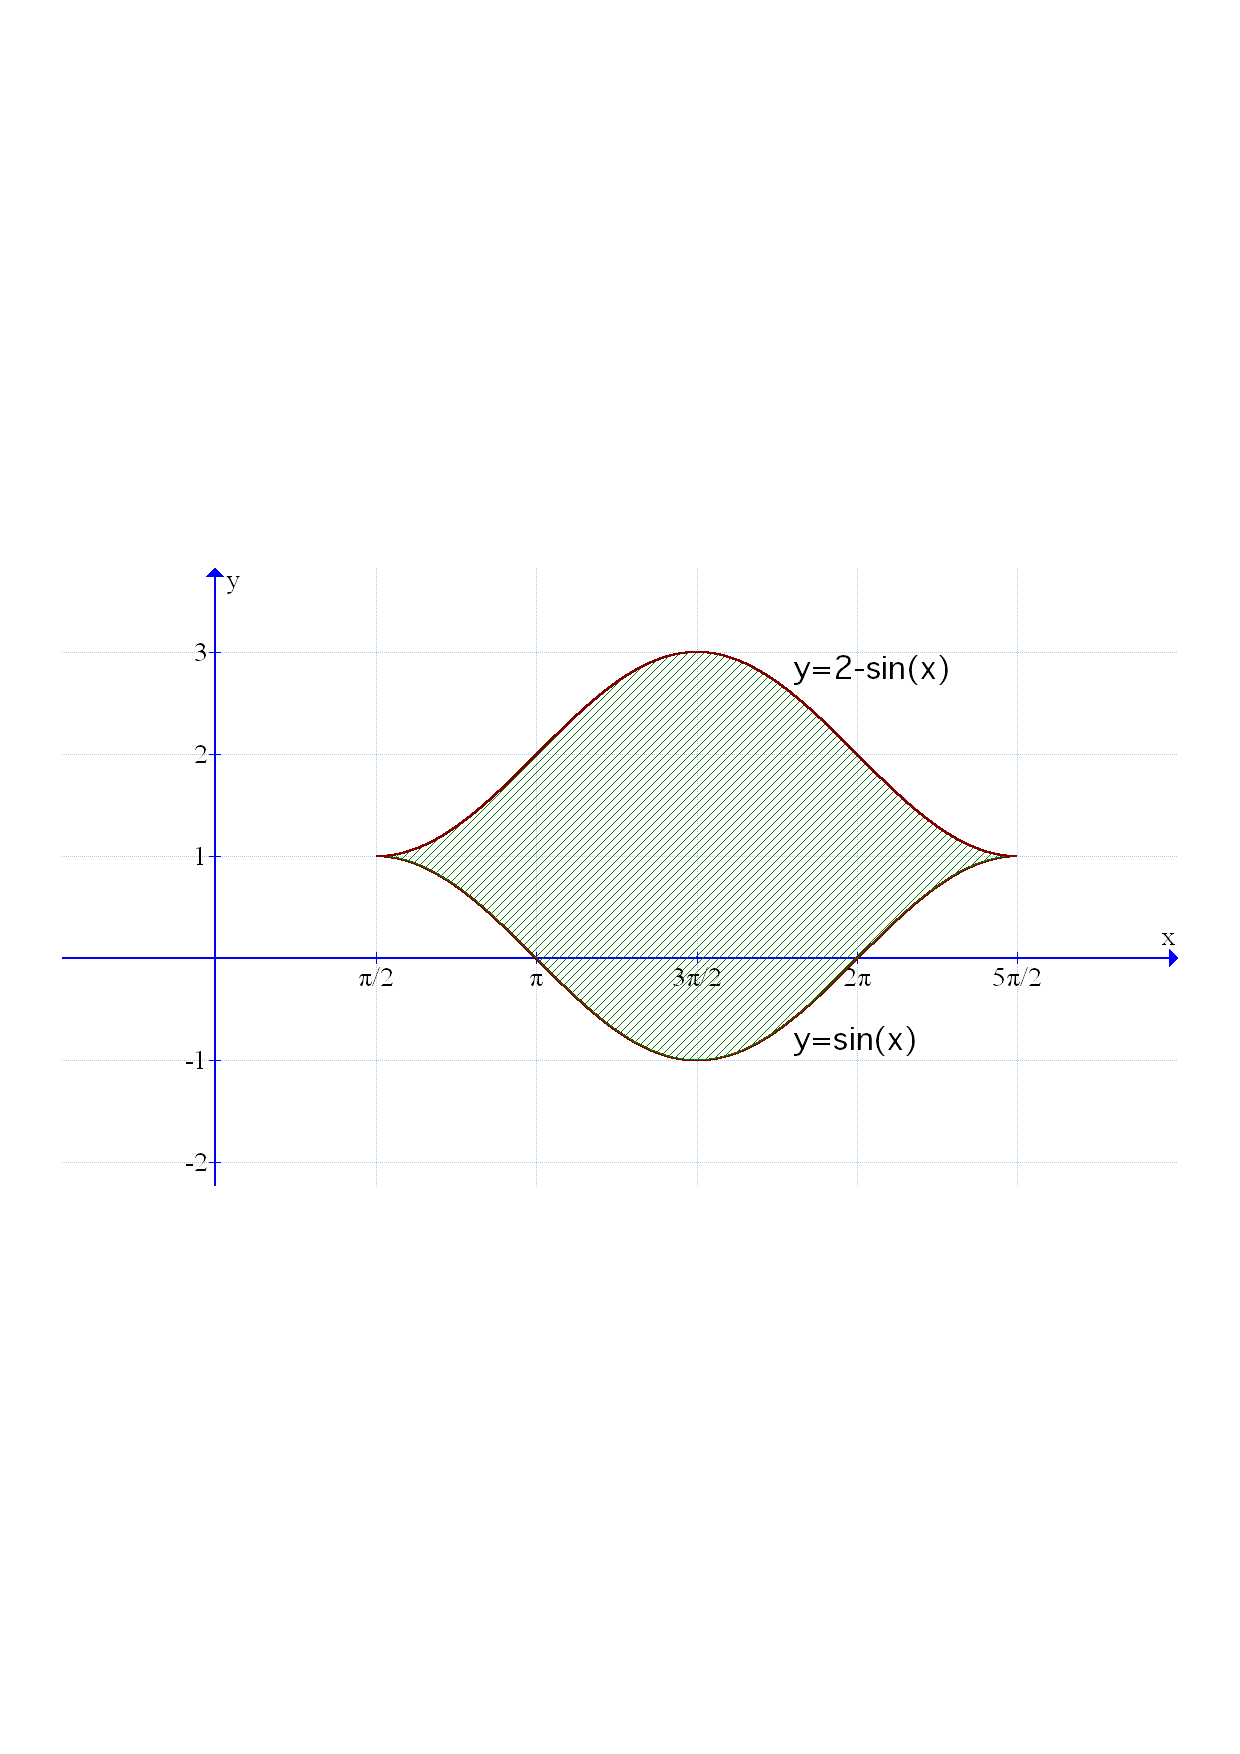
\includegraphics[scale=0.5]{lips.pdf}} \fi

\item Sketch the region in the $xy$-plane which is enclosed by $y=\sec{x}$ and $y=\frac{1}{2}$ for $-\frac{\pi}{4}\leq x \leq \frac{\pi}{4}$.

\ifans\fbox{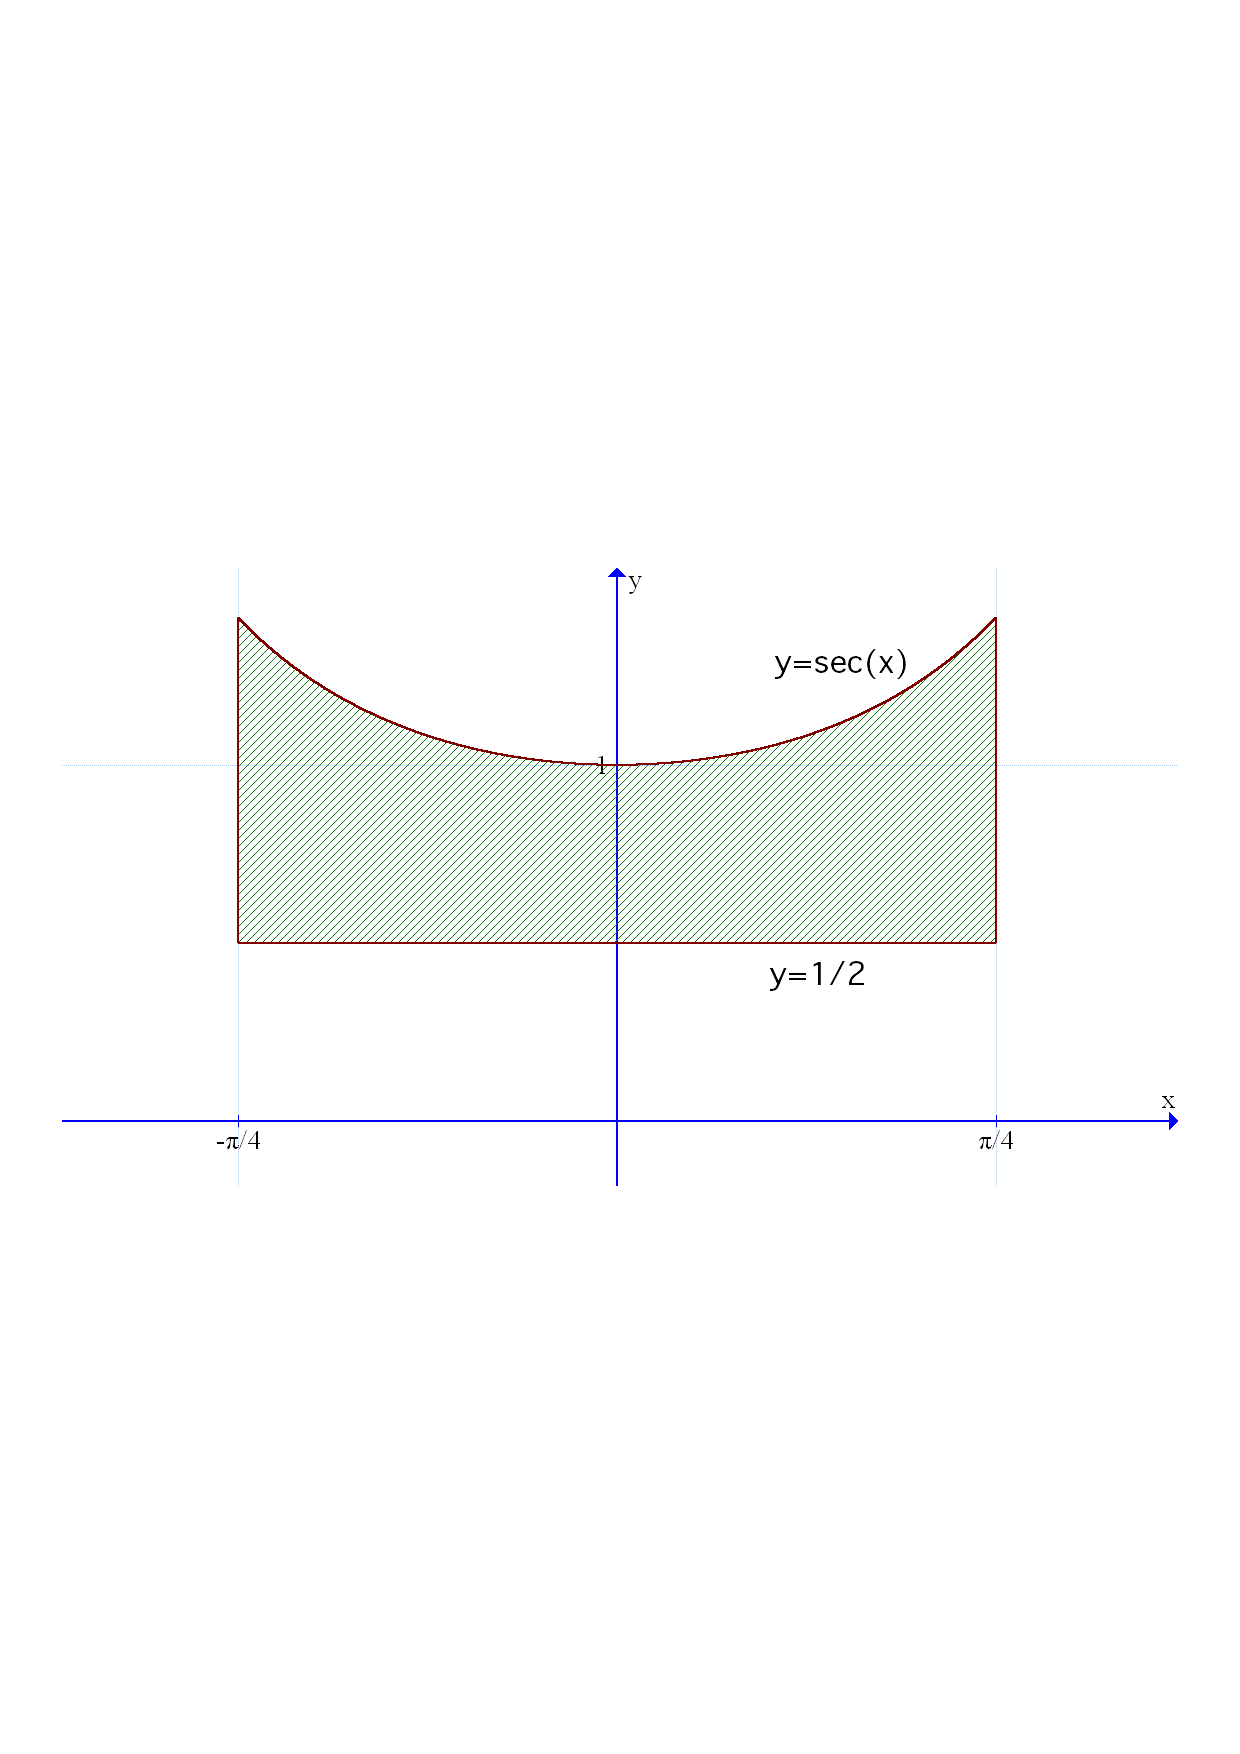
\includegraphics[scale=0.5]{sec_area.pdf}} \fi

\item Sketch $f(x) = \sin^2(x)$ on the interval $[0,2\pi]$.  Label all asymptotes, intercepts with the coordinate axes, and local extrema.\\
{\bf Hint:} $f^{\prime}(x) = 2\sin{x}\cos{x}$ and $f^{\prime\prime}(x)=4\cos^2{x}-2$

\ifans{\fbox{ 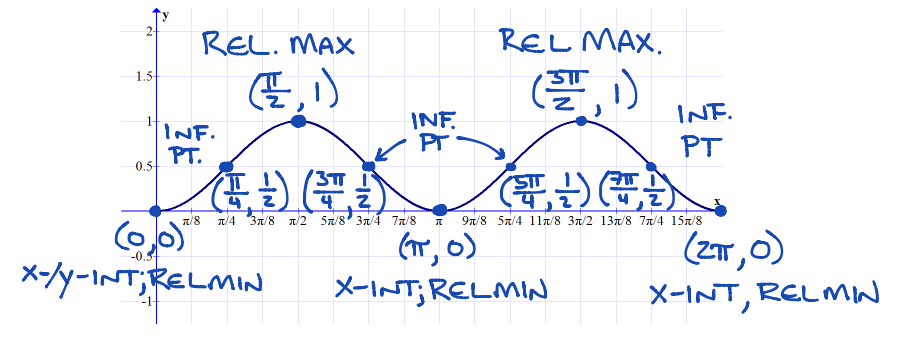
\includegraphics[scale=0.6]{SineSquared.png}}} \fi

\end{enumerate}

\end{document}